% !TEX encoding = UTF-8 Unicode
\documentclass[a4paper]{article}

\usepackage{color}
\usepackage{url}
\usepackage[T2A]{fontenc} % enable Cyrillic fonts
\usepackage[utf8]{inputenc} % make weird characters work
\usepackage{graphicx}
\usepackage{floatrow}
\usepackage{subcaption}
\usepackage[export]{adjustbox}
\usepackage{pgfplots}
\pgfplotsset{compat=1.3}

\pgfplotsset{%
    % #1: index in the group(0,1,2,...)
    % #2: number of plots of that group
    bar group size/.style 2 args={%
        /pgf/bar shift={%
                % total width = n*w + (n-1)*skip
                % -> subtract half for centering
                -0.5*(#2*\pgfplotbarwidth + (#2-1)*\pgfkeysvalueof{/pgfplots/bar group skip})  +
                % the '0.5*w' is for centering
                (.5+#1)*\pgfplotbarwidth + #1*\pgfkeysvalueof{/pgfplots/bar group skip}},%
    },
    bar group skip/.initial=2pt,
    plot 0/.style={blue,fill=blue!30!white,mark=none},%
    plot 1/.style={red,fill=red!30!white,mark=none},%
    plot 2/.style={brown!60!black,fill=brown!30!white,mark=none},%
    plot 3/.style={gray,fill=gray,mark=none},%
}

\usepackage[english,serbian]{babel}
%\usepackage[english,serbianc]{babel} %ukljuciti babel sa ovim opcijama, umesto gornjim, ukoliko se koristi cirilica

\usepackage[unicode]{hyperref}
\hypersetup{colorlinks,citecolor=green,filecolor=green,linkcolor=blue,urlcolor=blue}

\usepackage{listings}

%\newtheorem{primer}{Пример}[section] %ćirilični primer
\newtheorem{primer}{Primer}[section]

\definecolor{mygreen}{rgb}{0,0.6,0}
\definecolor{mygray}{rgb}{0.5,0.5,0.5}
\definecolor{mymauve}{rgb}{0.58,0,0.82}

\lstset{% 
  backgroundcolor=\color{white},   % choose the background color; you must add \usepackage{color} or \usepackage{xcolor}; should come as last argument
  basicstyle=\scriptsize\ttfamily,        % the size of the fonts that are used for the code
  breakatwhitespace=false,         % sets if automatic breaks should only happen at whitespace
  breaklines=true,                 % sets automatic line breaking
  captionpos=b,                    % sets the caption-position to bottom
  commentstyle=\color{mygreen},    % comment style
  deletekeywords={...},            % if you want to delete keywords from the given language
  escapeinside={\%*}{*)},          % if you want to add LaTeX within your code
  extendedchars=true,              % lets you use non-ASCII characters; for 8-bits encodings only, does not work with UTF-8
  firstnumber=1000,                % start line enumeration with line 1000
  frame=single,	                   % adds a frame around the code
  keepspaces=true,                 % keeps spaces in text, useful for keeping indentation of code (possibly needs columns=flexible)
  keywordstyle=\color{blue},       % keyword style
  language=Python,                 % the language of the code
  morekeywords={*,...},            % if you want to add more keywords to the set
  numbers=left,                    % where to put the line-numbers; possible values are (none, left, right)
  numbersep=5pt,                   % how far the line-numbers are from the code
  numberstyle=\tiny\color{mygray}, % the style that is used for the line-numbers
  rulecolor=\color{black},         % if not set, the frame-color may be changed on line-breaks within not-black text (e.g. comments (green here))
  showspaces=false,                % show spaces everywhere adding particular underscores; it overrides 'showstringspaces'
  showstringspaces=false,          % underline spaces within strings only
  showtabs=false,                  % show tabs within strings adding particular underscores
  stepnumber=2,                    % the step between two line-numbers. If it's 1, each line will be numbered
  stringstyle=\color{mymauve},     % string literal style
  tabsize=2,	                   % sets default tabsize to 2 spaces
  title=\lstname                   % show the filename of files included with \lstinputlisting; also try caption instead of title
}

\begin{document}

\title{Projekat GraalVM\\ \small{Seminarski rad u okviru kursa\\Metodologija stručnog i naučnog rada\\ Matematički fakultet}}

\author{Bojan Bardžić, Milica Gnjatović, Pavle Savić, Andrija Urošević\\ 
	\texttt{mi18300@alas.matf.bg.ac.rs}, 
	\texttt{mi18018@alas.matf.bg.ac.rs}, \\ 
	\texttt{pavlesavic1389@gmail.com}, 
	\texttt{mi18083@alas.matf.bg.ac.rs}}

%\date{9.~april 2015.}

\maketitle

\abstract{
U ovom tekstu je ukratko prikazana osnovna forma seminarskog rada. Obratite pažnju da je pored ove .pdf datoteke, u prilogu i odgovarajuća .tex datoteka, kao i .bib datoteka korišćena za generisanje literature. Na prvoj strani seminarskog rada su naslov, apstrakt i sadržaj, i to sve mora da stane na prvu stranu! Kako bi Vaš seminarski zadovoljio standarde i očekivanja, koristite uputstva i materijale sa predavanja na temu pisanja seminarskih radova. Ovo je samo šablon koji se odnosi na fizički izgled seminarskog rada (šablon koji \emph{morate} da koristite!) kao i par tehničkih pomoćnih uputstava. Pročitajte tekst pažljivo jer on sadrži i važne informacije vezane za zahteve obima i karakteristika seminarskog rada.}

\tableofcontents

\newpage

\section{Uvod}
\label{sec:uvod}
GraalVM je alat koji omogućava pisanje i izvršavanje koda u različitim jezicima\cite{graalvm}. GraalVM podržava naredne jezike: 
\begin{itemize}
	\item Java
	\item JavaScript i Node.js
	\item Python
	\item Ruby
	\item R
	\item LLVM jezici poput C-a i C++-a
	\item WebAssembly\\
	
U ovom radu ćemo proći kroz osnovne elemente i ciljeve ovog alata, šta je to inovativno uvedeno ovim projektom i gde se sve koristi. 
\end{itemize}

\subsection{Istorijski razvoj}
\label{subsec:Istorijski razvoj}

Projekat GraalVM je istraživački projekat koji razvija Oracle labs. Od 2012. preko šezdeset naučnih radova je izdato od strane razvojnog tima. Jedan od prvi radova koji iznose ideju ovog projekta je \textit{One VM to rule them all}. \cite{onevmtorulethemall} \\

Java Virtuelne mašine poput Oraklovog Java HotSpotVM i IBMov Java VM postoje već 20ak godina. Međutim nije postojala virtuelna mašina koja bi omogućila efikasno izvršavanje kodova pisanih u različitim jezicima. Cilj ovog projekta je bio da se napavi objedinjena virtuelna mašina koja bi ovo omogućila.\\

GraalVM 19.0 je objavljen u Maju 2019e i to je prva verzija ovog alata. Trenutno najnovija verzija je GraaLVM 22.1.0 objavljena u Aprilu 2022. \cite{graalvmreleases}



\subsection{Jedan alat - više jezika}


\begin{figure}
	\caption{Podržani jezici}
	\begin{subfigure}{\linewidth}
		
\includegraphics[width=0.16\linewidth]{imgs/java_logo.png}
		
\includegraphics[width=0.16\linewidth]{imgs/c_logo.png}
		
\includegraphics[width=0.16\linewidth]{imgs/cpp_logo.png}
		
\includegraphics[width=0.16\linewidth]{imgs/r_logo.png}
		
\includegraphics[width=0.16\linewidth]{imgs/python_logo.png}
		
\includegraphics[width=0.16\linewidth]{imgs/ruby_logo.png}
	\end{subfigure}
	
	\begin{center}
		
\includegraphics[width=0.5\linewidth]{imgs/graalvm_logo.png}	
	\end{center} 
	
	\begin{subfigure}{\linewidth}
		
\includegraphics[width=0.16\linewidth]{imgs/js_logo.png}
		
\includegraphics[width=0.16\linewidth]{imgs/nodejs_logo.png}
		
\includegraphics[width=0.16\linewidth]{imgs/clojure_logo.png}
		
\includegraphics[width=0.16\linewidth]{imgs/kotlin_logo.png}
		
\includegraphics[width=0.16\linewidth]{imgs/scala_logo.png}
		
\includegraphics[width=0.16\linewidth]{imgs/wa_logo.png}
	\end{subfigure}
	\label{podržani jezici}
\end{figure}
Korišćenjem ovog alata je omogućeno efikasnije korišćenje više jezika na jednom projektu. U projektu je moguće kodom jednog jezika pozivati funkcije pisane u drugom jeziku. Dopušteno je deljenje struktura podataka između kodova pisanih u različitim jezicima. Na ovaj način je omogućeno da sakupljač otpadaka radi na celom projektu bez obzira na to koliko različitih jezika je korišćeno. Ovim je omogućeno i jednostavnije debagovanje.\\

Ovaj alat je koristan u radu sa mikroservisnom arhitekturom. Nekolicina okvira za rad sa Java mikroservisima je već prihvatila ovu platformu. Između ostalih to su Micronaut, Spring, Helidon i Quarkus. 

Još jedna od mogućnosti koje GraalVM nudi je implemenitranje novih jezika i alata korišćenjem biblioteke Truffle.

GraalVM je implementiran u javi. Čine ga Java Virtuelna Mašina - JVM i Java Development Kit - JDK. \\
Ovaj alat omogućava brže izvršavanje koda, a da se pri tome koristi manje memorije.

GraalVM je dostupan na Linux, Windows i macOS operativnim sistemima. \\

Dostupna su dva izdanja GraalVM-a:

\begin{description}
	\item [Community eddition] je otvorenog koda i dostupno je u \href{https://github.com/oracle/graal}{github repozitorijumu}. Korisnici mogu doprineti razvoju ove verzije kreiranjem githb issue-a i pravljenjem pull request-ova. \cite{graalvmCommunity}
	\item [Enterprise eddition] razvija i licensira kompanija Oracle. \cite{graalvmEnterprise}
\end{description}

GraalVM podržavaju razvojna okruženja i protokoli za debagovanje. Neka od podržanih okruženja su Eclipse, NetBeans, IntellliJ IDEA i Visual Studio Code. Ova okruženja su posebno dobra jer podržaju sve jezike koje podržava i GraalVM. Ovaj alat obezbeđuje ugrađen Crome DevTools Protocol, Debug Adapter Protocol (DAP) i Language Server Protocol (LSP), čime je omogućeno debagovanje JavaScript, R i Ruby kodova.

\section{Šta obuhvata projekat?}
\label{sec:Šta obuhvata projekat?}
Kao što je prethodno navedeno, ovaj projekat uvodi neke nove koncepte.
Sam projekat obuhvata više komponenti koje ga čine korisnim i inovativnim.

\subsection{GraalVM kao zamena za JVM}
\label{sub:GraalVM kao zamena za JVM}

Jedna od prednosti GraalVM je što se može koristiti umesto Java virtuelne mašine, on može da pokreće Javu, Skalu, Kotlin i sve ostale jezike koje se prevode u Java bajt kod. Od 2019. može se izvršavati na Linux-u, a od verzije 20.1.0 ima podršku i za Windows. \\

Još jedna od prednosti koja se pripisuje GraalVM-u su odlične performanse, neke demonstracije pokazuju da Ruby program izvršava i do 30 puta brže od originalne implementacije.
Detaljnija testiranja su ipak pokazala da se u proseku Ruby kod izvšava oko 30\%  brže na GraalVM, što je i dalje obećavajući rezultat. \\

Kada su testirani Java programi rezultati su bili manje optimistični, performanse GraalVM-a su okvirno slične Oracle-ovom HotSpot kompajleru. Ovo samo po sebi ne predstavlja loš rezultat, ali ne predstavlja ni neki revolucionarni napredak u odnosu na sadašnje tehnologije.U svakom slučaju, GraalVM će biti brži od klaične JVM. Iako ne predstavlja poboljšanje u odnosu na HotSpot VM, prednost GraalVM-a je u tome što je nov kompajler nad kojim nije vršena optimizacija preko dvadeset godina, kao što je to slučaj sa HotSpot-om. Još jedna prednost u odnosu na prethodne kompajlere je to što je pisan u Javi za razliku od prethodnih kompajlera koji su pisani u jezicima C i C++, to omogućava lakše proširenje i optimizaciju od strane Java programera.

\subsection{Truffle - kompajler za kompajlere}
\label{Truffle - kompajler za kompajlere}

Truffle je biblioteka otvorenog koda za pravljenje alata i implementacija programskih jezika kao interpretera za samomodifikujuća apstraktna sintaksna stabla. On nam dozvoljava 
da pravimo interpretere bez većih problema, ali prednost njegovog korišćenja je u tome što se interpretirani kod izvršava podjednako brzo kao i kompajlirani kod.
On je korišćen za pisanje interpretera za jezik JavaScrpit u GraalVM-u. Pri izvršavanju koda potrebno mu je neko vreme da se zagreje, ali kada dostigne optimalne performanse
one su okvirno iste kao V8 kompajler kompanije Google. \\

Sama optimizacija koda je zasnovana ideji parcijalne evaluacije. Truffle uzima interpreter koji smo mu dali i naš program i koristi JIT kompajler i promene sintaksnog stabla da izvrši optimizacije u našem kodu. Da bi se utvrdilo koje optimizacije je potrebno izvršiti program mora prvo biti pokrenut i zbog toga se javlja sporije vreme izvršavanja na početku.\\

 Takođe, pri pisanju interpretera koristeći Truffle možemo da naglasimo gde i kada želimo da kod bude optimizovan. U nekim slučajevima promena u izvornom kodu može da dovede do greške u programu i u tom slučaju je potrebno deoptimizovati kod. Sve ove optimizacije i izbacivanja nekorišćenog koda iz našeg programa dovode do velike brzine izvršavanja. \\

Standardni podržani jezici za Truffle su JavaScript sa okruženjem Node.js ugrađenim u njega, kao i Ruby, R i Python. Pored toga, Truffle ima u sebe ugrađen Sulong koji može da izvršava LLVM bitkod i tako izvšava programe pisane na jezicima kao što su C, C++, C\#, D, Lua i FORTRAN. Ovim omogućavamo da GraalVM izvšrava veliki broj različitih programskih jezika kao i da se funkcije iz jednog jezika pozivaju u drugom jeziku omogućavajući veću fleksibilnost pri pisanju programa.

\subsection{Izvršavanje mašinskog koda na klaudu}
\label{sub:Izvršavanje mašinskog koda na klaudu}

Jedna od glavnih funkcionalnosti koje uvodi ovaj projekat jeste kompajliranje Java programa sa bajt koda na mašinski kod. Ovo je novina koja nam dozvoljava tako nešto prvi put od kako postoji programski jezik Java. Jedan od slučajeva upotrebe za ovo je izvšavanje mikroservisa na klaudu. \\

Mikroservisi se sada kompajliraju u izvršni fajl i time je eliminisana potrebna da na serverskoj strani mora postojati Java virtuelna mašina, što dovodi do smanjenja zauzeća memorije na serveru. Još jedna prednost ovog pristupa je u tome što više nije potrebno da se za naše programe učitava mnoštvo Java klasa pri pokretanju, od kojih većina neće biti upotrebljeno. Ovo dovodi do bržeg izvršavanja naših programa na serverskoj strani i sprečava sporo izvšavanje pri prvom pokretanju. 


\begin{figure}
	\begin{center}
	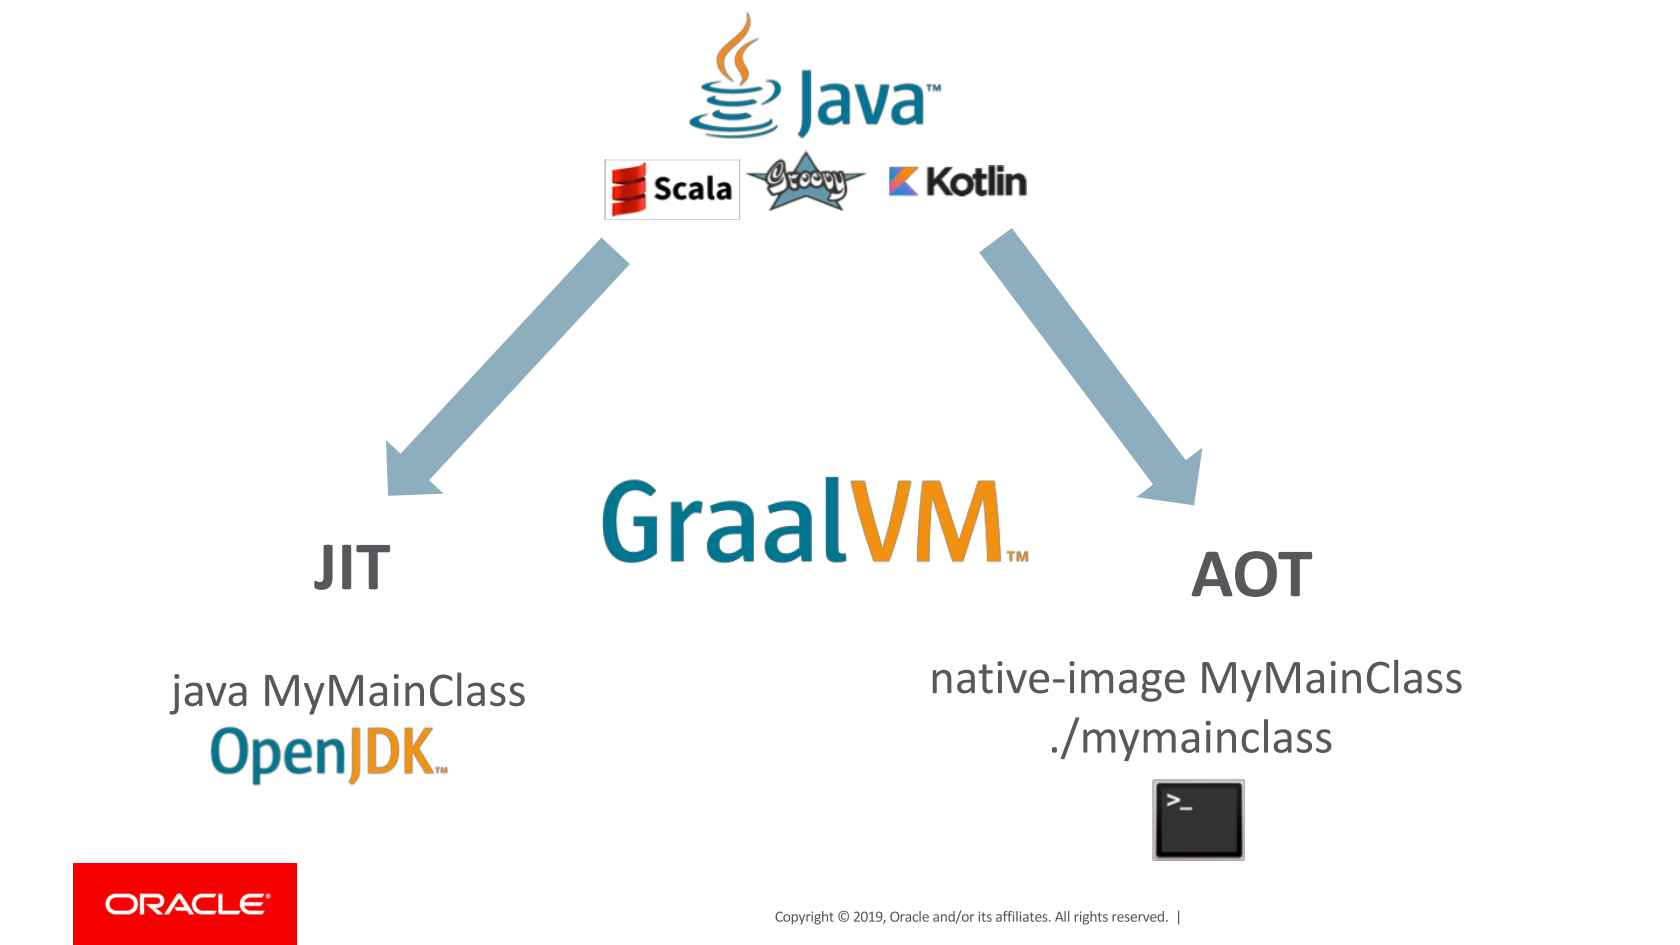
\includegraphics[scale=0.25]{imgs/run_java.jpg}
	\end{center}
	\caption{Dva načina za pokretanje Java programa korišćenjem GraalVM-a}
	\label{fig:run java}
\end{figure}


\subsection{Espresso - Java on Truffle}
\label{sub:Espresso - Java on Truffle}

Pored dva ustaljena načina za pokretanje koda napisanog u Java-i korišćenjem GraalVM-a od verzije 21.0 uvedena je nova komponenta, nazvana \emph{espresso}, koja predstavlja implementaciju JVM specifikacije, napisanu u Java-i, pomoću Truffle radnog okvira. Ova komponenta nije podrazumevano deo GraalVM-a ali može se lako instalirati korišćenjem \emph{GraalVM Updater tool}-a. Na raspolaganju je i za GraalVM distribucije zasnovane na Java-i 8, kao i na Java-i 11 tako da se može koristiti kao zamena za JVM po izboru. \\


\emph{Java on Truffle} režim izvršavanja pokreće Java kod preko bajtkod interpretera implementiranog korišćenjem Truffle-a. Na ovaj način Java (i drugi JVM zasnovani jezici) pokreću se na isti način kao tradicionalni interpretirani i LLVM jezici koje GraalVM podržava što omogućava potpunu interoperabilnost sa njima. Iz tog razloga se mogu pozivati f-je napisane u ovim jezicima u Java-i, kao i Java f-je u drugim Truffle jezicima i razmenjivati podaci u zajedničkom memorijskom prostoru (\emph{polyglot} programi). Pored toga mogu se iskoristiti alati koje Truffle nudi, a koji nisu dostupni za Java-u. \\

Činjenica da je \emph{Java on Truffle} implementiran u Java-i (eng. \emph{self-hosting} smatra se \emph{Svetim gralom} u razvoju JVM-a. Kao implementacija JVM-a, da bi \emph{Java on Truffle} mogla da pokrene Java kod neophodan joj je pristup JCL-u (Java Class Library) i nativnim bibliotekama i metodama koje pruža JDK (Java Development Kit). \emph{Java on Truffle} ponovno koristi Java Archive datoteke i nativne biblioteke iz GraalVM distribucije. Kao posledica \emph{self-hosting}-a \emph{Java on Truffle} jeste metacirkularna VM - može pokretati samu sebe nekoliko nivoa u dubinu (pri čemu svakim silaskom u dubinu postaje nešto sporija). Druga prednost ovoga je da je izvorni kod razumljiv Java programerima. Ovaj nivo transparentnosti, kroz zajednicu otvorenog koda, čini \emph{Java on Truffle} projektom koji se ubrzano razvija i unapređuje. \\

\emph{Java on Truffle} istovremeno je JVM i Java program, što znači da može biti pokrenuta unutar drugog Java programa. Ovo daje mogućnost razdvajanja aplikacije u komponente sa zajedničkom funkcionalnošću kako bi se proces programiranja učinio lakšim za upravljanje i podigla ponovna upotrebljivost koda. Na ovaj način može se ugraditi Java 8 kontekst u Java 11 aplikaciju i obrnuto, koristeći \emph{GraalVM Polyglot API}. Na primer ako su na raspolaganju obe distribucije (JDK 11 i JDK 8), \emph{Java on Truffle} može biti pokrenuta kao Java 8 aplikacija, a potom biti iskorišćena za pokretanje Java 11 bajtkoda i obrnuto. Ako postoji biblioteka dostupna samo za Java-u 8, sada je moguće prebaciti se na noviji JDK i, uz manje programerske napore da se upostavi interoperabilnost, koristiti je u Java 11 aplikaciji. Takođe ovime se povećava nivo izolovanosti \emph{host} VM-a i Java programa koji se pokreće što je iz bezbednosnih razloga značajno (može se pokretati i manje pouzdan ili nepoznat kod). \\


\begin{figure}
	\begin{center}
	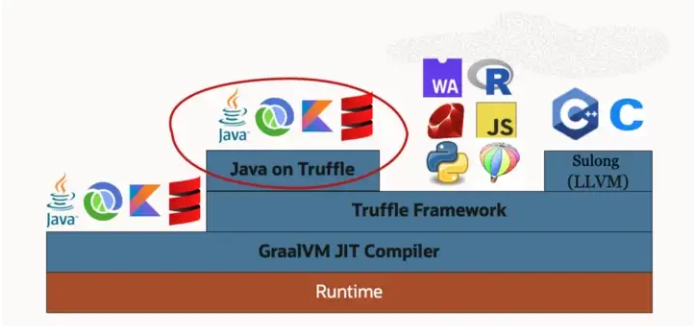
\includegraphics[scale=0.35]{imgs/java_on_truffle.png}
	\end{center}
	\caption{\emph{Java on Truffle} u GraalVM ekosistemu}
	\label{fig: java on truffle}
\end{figure}



\section{Karakteristike}
\label{sec:Karakteristike}

Projekat \emph{GraalVM} karakterišu visoke performanse, poliglot programiranje, \emph{GraalVM AOT} (\emph{ahead-of-time}) kompilacija u \emph{Native Image}, napredni alati\cite{graalvm}. U narednim pod sekcijama će biti opisani svaki od ovih karakteristika.

\subsection{Visoke performanse}
\label{sub:perf}

Jedna od karakteristika kojom \emph{GraalVM} može da se pohvali, jestu veoma visoke performanse u odnosu na \emph{OracleJDK}, i \emph{OpenJDK}. 

Šipek i drugi \cite{vsipek19} pokretanjem \emph{DaCapo} benčmarka \cite{dacapo} pokazuju da \emph{GraalVM CE}, i posebno \emph{GraalVM EE} daju bolje performanse u odnosu na \emph{JDK10} i \emph{JDK11} (slika~\ref{fig:dacapo}). Na testu h2 \emph{GraalVM CE} daje rezultate i za 19.8\% bolje od \emph{JDK11}. Na drugim testovima vidimo malo poboljšanje \emph{GraalVM} kompajlera u odnosu na \emph{JDK}, ali i to da \emph{JDK} u malom broju testova daje bolje rezultate. Pored toga, treba uočavamo da \emph{GraalVM EE} u odnosu na \emph{GraalVM CE} nad h2 testovima daje rezultate bolje i za 47.06\%, što je veoma velika razlika. Što se stabilnosti tiče, tj.\ veličine standardne devijacije u performansam, najbolje se pokazuje \emph{JDK11}, a najgore \emph{GraalVM EE}.

\begin{figure}
\begin{center}
    \begin{tikzpicture}
    \begin{axis}[
        width=0.85\textwidth,
        x tick label style={/pgf/number format/1000 sep=},
        ylabel=Prosečno vreme u $ms$,
        enlargelimits=0.15,
        legend style={at={(0.5,-0.15)},
        anchor=north,legend columns=-1},
        ybar,
        bar width=7pt,
        xtick={0,1,2,3,4,5},
        xticklabels={h2, lusearch, xalan, pmd, sunflow, jython},
        ]
        \addplot[plot 0,bar group size={0}{4}]
        coordinates {(0,4494.95) (1,2683.40) (2,863.32) (3,138.23) (4,5062.05) (5,6652.86)};
        \addplot[plot 1,bar group size={1}{4}]
        coordinates {(0,5327.10) (1,2757.10) (2,277.41) (3,194.61) (4,5626.25) (5,7038.34)};
        \addplot[plot 2,bar group size={2}{4}]
        coordinates {(0,10821.85) (1,2874.50) (2,870.72) (3,201.95) (4,5417.25) (5,6433.60)};
        \addplot[plot 3,bar group size={3}{4}]
        coordinates {(0,9550.05) (1,2886.15) (2,232.51) (3,276.76) (4,6151.25) (5,6672.10)};
        \legend{GraalVM EE, GraalVM CE, JDK10, JDK11}
    \end{axis}
\end{tikzpicture}
\end{center}
    \caption{\emph{DaCapo} benčmark na \emph{GraalVM EE, GraalVM CE, JKD10, JDK11}}
\label{fig:dacapo}
\end{figure}

Pored \emph{DaCapo} benčmarka razvija se i novi \emph{Renaissance} benčmark. \emph{Renaissance} benčmark obećava prednosti nad konkurencijom, tako što koristi moderna, realna, konkurentna, i objektno orijentisana preopterećenja kako bi prikazao bolju sliku performansi kompajlera \cite{prokopec19}. Pokretanjem ovih testova uočeno je značajno poboljšanje \emph{GraalVM JIT} kompajlera u odnosu na \emph{JDK11} i \emph{JDK17} \cite{renaissance}.

Poboljšanje u performansama je vidljivo i na drugim benčmarkovima. Tako je uočeno da \emph{Scala} ima bolje performanse kada se koristi \emph{GraalVM} optimizator, takođe na \emph{DaCapo} benčmarkovima \cite{stadler13, dacapo}. Claud servisi, takođe, dobijaju značajno unapređenje \cite{sipek21}. 

Treba napomenuti da postoje istraživanja koja pokazuju da \emph{GraalVM} ne pokazuje značajna poboljšanja u odnosu na \emph{JKD}. Fong i drugi \cite{fong21} pokazuju da u nekim slučajevima \emph{GraalVM} daje podjednake čak i lošije rezultate. 

\subsection{Native Image}
\label{sub:nim}

\emph{GraalVM} pruža tehnologiju \emph{Native Image} \cite{graalvm}. \emph{Native Image} predstavlja izvršivi binarni fajl koji je dobijen \emph{GraalVM AOT} kompajlerom. Ovaj fajl sadrži klase aplikacije, klase biblioteka, zavisne klase i statički linkovan kod iz \emph{JDK}-a. Dobijeni izvršivi fajl se ne pokreće na \emph{Java VM}, već on uključuje potrebne dodatke iz \emph{Java VM}-e. Za rezultat imamo to da se dobijeni program pokreće brže, jer učitava samo potrebne klase. Program je sigurniji, jer se sa manjom bazom koda mogućnost nastanka baga smanjuje. Program se lako dostavlja, jer se kapacitet kontejnera smanjuje.

\subsection{Poliglot programiranje}
\label{sub:poliglot}

Jedna od ključnih karakteristika koju \emph{GraalVM} pruža jeste poliglot programiranje \cite{graalvm}. Poliglot programiranje podrazumeva da programeri za rešavanje neko problema koriste odgovarajući programski jezik. Tako rešene probleme onda koriste u projektu. Mehanizmi integracije više programskih jezika stvara dodatne kompleksnosti. Postoje mnogi radovi koji tvrde da se efikasnost programera, samim tim i programa smanjuje uvođenjem više jezičke strukture \cite{peterson21, hao20}. Sa ciljem rešavanja ovog problema \emph{GraalVM} pruža \emph{TruffleVM} koji obećava lako i jednostavno prenošenje podataka, i korišćenje konstrukcija nekog programskog jezika unutar nekog drugog programskog jezika \cite{grimmer15}.

\subsection{Napredni alati}
\label{sub:alati}

U tabeli~\ref{alati} su prikazani dostupni alati i njihove funkcionalnosti unutar projekta \emph{GraalVM} \cite{graalvm}.

\begin{table}
    \centering
    \begin{tabular}{|l|l|}
        \hline
        VS Code Extensions & Radno okruženje unutar VS Code-a\\
        \hline
        GraalVM Dashboard & Vizualna reprezentacija delova\\
        \hline
        Chrome Debugger & Debager za JS, Ruby, R i Python\\
        \hline
        VisualVM & Profajler, monitor, aktivni tredovi\ldots\\
        \hline
        GraalVM Insight & Praćenje programa u izvršavanju\\
        \hline
        Ideal Graph Visualizer & Faze kompilacije\\
        \hline
    \end{tabular}
    \caption{Napredni alati unutar Projekta \emph{GraalVM}}
    \label{alati}
\end{table}


\section{Kompanije koje koriste GraalVM}
\begin{description}
	\item[Facebook] \hfill \\
	Društvena mreža Facebook ima ogroman broj korisnika zbog čega je jako bitno da se kod dobro skalira i brzo izvršava.
	Na serverskoj strani koristi Javu i Spark framework za rad sa velikom količnimo podataka. Prelazak sa Oracle JDK-a i Open JDK-a na GraalVM se sveo samo na promenu runtime okruženja, bez ikakvih promena u kodu. Izmereno je prosečno ubrzanje 1.1x korišćenjem Community verzije i ubrzanje 1.42x korišćenjem Enterprise verzije GraalVM-a. \cite{graalvmusecases}
	
	\item[Twitter] \hfill \\
	Kao i Facebook, Twiter je društvena mreža sa milionima korisnika. Sa porastom broja korisnika bile su neophodne promene koje bi omogućile brzo izvršavanje uz minimalne troškove. Većina mikroservisa tvitera je implementirano u Skali. Prelaskom na GraalVM je omogućeno 8-11\% ušteda na procesoru. \cite{graalvmusecases}	
	
	\item[Standard Chartered Bank] \hfil \\
	Ova kompanija je između ostalog koristila Javu, Python sa SpringBoot okvirom kako bi obezbedila stabilnost i robusnost programa. Pre par godina kompanije je odlučila da svoju aplikaciju prebaci u cloud, što je donelo nove izazove. GraalVM je obezbedio jednostavan prelazak na cloud time što podržava tehnologije koje su programi već koristili. GraalVM je omogućio skalabilnost i ubrzanje od 7\%.\cite{graalvmusecases}
		
	\item[Goldman Sachs]  \hfil \\
	Goldman Sachs je investiciona banka. Ova kompanija ima svoj programski jezik Slang koji ima funkcije pogodne za njiove potrebe. Jezik je dosta glomazan i potrebno mu je unapređenje. Prevođenje celog koda u neki drugi jezik bi bilo previše zahtevno. GraalVM i Truffle su omogućili unapređenje i ubrzanje izvršavanja koda pisanog u Slangu, a da je pri tom napisana minimalna količina novog koda.\cite{graalvmusecases}
	
	\item[Nvidia]  \hfil \\
	Nvdia je jedan od najvećih proizvođača grafičkih kartica. Iako neki jezici jednostavno mogu da ubrzaju izvršavanje korišćenjem grafičke katice, za neke druge to može biti izazovno. GraalVM i Truffle su omogućili kreiranje grCuda jezika koji je kao dodatni jezik GraalVM. Kako jezici u GraalVM efikasno komuniciraju međusobno tako je omogućna jednostavna komunikacija sa jezikom grafičke kartice i samom grafičkom.\cite{graalvmusecases}
	
	\item[Politie]  \hfil \\
	Holandska policija je imala monolitnu aplikaciju koja je koristila između ostalog TypeScrip, Angular, Scala, Axon, SpringBoot, Slick i R. Ova aplikacija je obrađivala velike količine podataka u realnom vremenu, ali to je bilo veoma sporo. Cilj je bio preći u cloud i na mikroservisnu ahitekturu, a pri tom ne implemenitrati sve iz početka. GraalVM je omogućio ovaj prelazak i ubrzanje, pri čemu je ostao značajan deo starog koda.\cite{graalvmusecases}
	
\end{description}


\section{Zaključak}
\label{sec:zakljucak}
GraalVM je u ovom radu predstavljen kao nešto izuzetno korisno i efikasno. Dalje se postavlja pitanje `Da li GraalVM ima konkurenciju?'.

Trenutno nema projekata sličnih ovome. Prema tome, glavna konkurencija ostaju kompajleri i alati za pojedinčna jezike. Danas se kao glavna konkurncija navode Amazon Coretto, Red Hat, OpenJDK, Azul Platform Prime i Microsoft Build of OpenJDK. 

\addcontentsline{toc}{section}{Literatura}
\appendix
\bibliography{seminarski} 
\bibliographystyle{plain}

\end{document}
